\documentclass[12pt]{article}
\usepackage[a4paper, total={5.5in, 9in}]{geometry}
\usepackage{amsmath}
\usepackage{changepage}
\usepackage[most]{tcolorbox}
\usepackage{textcomp}
\usepackage{tikz}
\usepackage{pgfplots}
\pgfplotsset{compat=1.18}
\usepackage{amsfonts}
\usepackage{graphicx}

\newcommand{\ihat}{\boldsymbol{\hat{\textbf{\i}}}}
\newcommand{\jhat}{\boldsymbol{\hat{\textbf{\j}}}}


\title{Precalculus Worksheet 8.8}
\author{PCL Learning Center}
\date{}

\begin{document}
\maketitle
\begin{center}
    \textit{note: This worksheet may be used for two sessions, and\\no electronic devices may be used on this worksheet.}
\end{center}

\section*{Problem Set 1\\Difficulty level: Normal}
\subsection*{Problem 1}
Given the points \(P(4,9)\) and \(Q(8,9)\), find the magnitude and direction of \( \overrightarrow{PQ}\).

\subsection*{Problem 2}
Given the vector \(\vec{u}=\langle 5\sqrt{2},-5\sqrt{2} \rangle \), find the magnitude and direction of \(\vec{u}\).

\subsection*{Problem 3}
Given vectors \(\vec{u} = \langle 38, -5 \rangle\) and \(\vec{v} = \langle -40, 33 \rangle\), find the vector \(\vec{u} - \vec{v}\).

\subsection*{Problem 4}
Let \(\vec{u} = \langle -3, 2 \rangle\) and \(\vec{v} = \langle -8, -2 \rangle\). Find \(\vec{u} + \vec{v}\).

\subsection*{Problem 5}
Given \(\vec{w} = \langle -8, -8 \rangle\), find \(5\vec{w}\).

\subsection*{Problem 6}
If \(\vec{u} = \langle -8, -20 \rangle\) and \(\vec{w} = \langle -3, -1 \rangle\), find \(\dfrac{1}{4} \vec{u} - 6\vec{w}\).

\newpage
\subsection*{Problem 7}
What is the position of the vector shown below?

\begin{figure}[!ht]
    \centering
    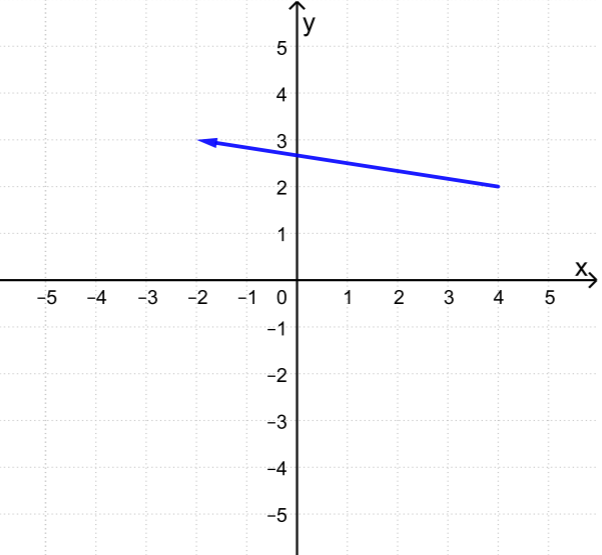
\includegraphics[width=0.7\linewidth]{vector_7.png}
\end{figure}

\subsection*{Problem 8}
The vector \( \overrightarrow{PQ}\) has initial point \(P(3,6)\) and position vector \(\langle 2,5 \rangle \). What are the coordinates of terminal point \(Q\)?

\subsection*{Problem 9}
Given a vector \(v\) with initial point \(P(36,7)\) and terminal point \(Q(14,-34)\), write the vector in terms of the unit vectors \(i\) and \(j\).

\subsection*{Problem 10}
Find a unit vector in the same direction as \( \vec{v} = \langle 5, 12 \rangle \).

\subsection*{Problem 11}
Given vectors \( \vec{u} = 5i - 29j \) and \( \vec{v} = 35i + 22j \), find vector \( \vec{u} - \vec{v} \).

\subsection*{Problem 12}
Given vectors \( \vec{u} = \langle -1, -8 \rangle \) and \( \vec{v} = \langle 1, 7 \rangle \), find \( \vec{u} \cdot \vec{v} \).

\subsection*{Problem 13}
Given \( \vec{u} = \langle 7, 5 \rangle \) and \( \vec{v} = \langle 8, -8 \rangle \), find the dot product \( \vec{u} \cdot \vec{v} \).

\subsection*{Problem 14}
Find the angle between \( \vec{u} = \langle -4, -3 \rangle \) and \( \vec{v} = \langle 4, -3 \rangle \).

\section*{Problem Set 2\\Difficulty level: Hard}
\subsection*{Problem 1}
How is a vector more specific than a line segment?

\subsection*{Problem 2}
What are \(\ihat\) and \(\jhat\), and what do they represent?

\subsection*{Problem 3}
What is component form?

\newpage
\section*{Solutions for the Set 1}
\subsection*{Problem 1}
\( |\overrightarrow{PQ}|=4, \theta =0^{\circ}\)
\subsection*{Problem 2}
\(|\vec{u}|=10,\theta=-45^{\circ}\)
\subsection*{Problem 3}
\((78,-38)\)
\subsection*{Problem 4}
\(\langle -11,0 \rangle\)
\subsection*{Problem 5}
\((-40,40)\)
\subsection*{Problem 6}
\(\langle 16,1 \rangle\)
\subsection*{Problem 7}
\(\langle -6, 1 \rangle \)
\subsection*{Problem 8}
\((5,11)\)

\subsection*{Problem 9}
\(\vec{v}=22\ihat -41\jhat\)
\subsection*{Problem 10}
\((\dfrac{5}{13},\dfrac{12}{13})\)
\subsection*{Problem 11}
\(-30\ihat-51\jhat\)
\subsection*{Problem 12}
\(-57\)
\subsection*{Problem 13}
16
\subsection*{Problem 14}
\(106.3^{\circ}\)
\section*{Solutions for the Set 2}
\subsection*{Problem 1}
A vector is a specific quantity drawn as a line segment with an arrowhead at one end. It has an initial point, where it begins, and a terminal point, where it ends. A vector is defined by its magnitude, or the length of the line, and its direction, indicated by an arrowhead at the terminal point.

\subsection*{Problem 2}
Are the unit vectors in the Cartesian coordinate system. The \(\ihat\) points in the direction of the \(x-\)axis, and the \(\jhat\) points in the direction of the \(y-\)axis.
\subsection*{Problem 3}
When we break a vector into two or more parts, each of those new vectors is a component of the original vector.

\end{document}
